\section{Analysis of the Reports}
\label{sec:analysis}

\Cref{tab:human} reports scores from a single rater. These ratings are thus subjective and tied to that rater's judgment. However, there are twenty reports on ten motions under consideration (ten \sys{} reports and ten STORM reports on the same motions), allowing us to assess them without a rater. The ten \sys{} and ten STORM reports are measured using the same procedures on each motion, and comparing them motion-by-motion controls for motion difficulty. We did not keep the Deep Research set, so we only compare \sys{} and STORM here. All reported differences are medians of motion-wise differences, with 95\% bootstrap intervals \citep{efron1993bootstrap} and Wilcoxon signed-rank tests \citep{wilcoxon1945}. With only ten motion pairs, the smallest attainable two-sided $p$-value is 0.002. (We strip bibliographies, headings, and markup before counting.)

\begin{table}[t]
\centering
\small
\resizebox{\linewidth}{!}{\begin{tabular}{lrrrrc}
\toprule
Measure & \sys{} & STORM & Difference & 95\% CI & Wins \\
\midrule
Citations per 100 words & 5.7 & 4.7 & $+$1.0 & [$+$0.0, $+$2.1] & 8/10 \\
Sentences with a citation & 0.46 & 0.60 & $-$0.15 & [$-$0.23, $-$0.09] & 0/10 \\
Distinct sources & 8 & 27 & $-$18 & [$-$24, $-$14] & 0/10 \\
Citations per source & 9.3 & 4.1 & $+$5.0 & [$+$1.7, $+$7.2] & 10/10 \\
Hedges per 1,000 words & 2.8 & 6.4 & $-$2.2 & [$-$7.3, $-$0.4] & 1/10 \\
Contrast markers per 1,000 words & 5.5 & 6.0 & $-$0.3 & [$-$0.8, $+$1.0] & 4/10 \\
Commitment markers per 1,000 words & 6.8 & 3.8 & $+$3.3 & [$+$0.4, $+$4.2] & 10/10 \\
Causal connectives per 1,000 words & 4.2 & 3.0 & $+$0.3 & [$-$0.5, $+$1.8] & 5/10 \\
Words & 1339 & 2426 & $-$1172 & [$-$1621, $-$617] & 0/10 \\
\bottomrule
\end{tabular}
}
\caption{\sys{} vs.\ STORM paired comparison. Values are medians over motions, computed from the ten \sys{} reports and ten STORM reports. Reported difference is the median over motions of motion-wise differences (along with a 95\% bootstrap interval). ``Wins'' indicates how many motions for which the \sys{} score is higher. The reported rates are based on the word lists in \Cref{app:lexicon}.}
\label{tab:text}
\end{table}

\begin{figure}[t]
\centering
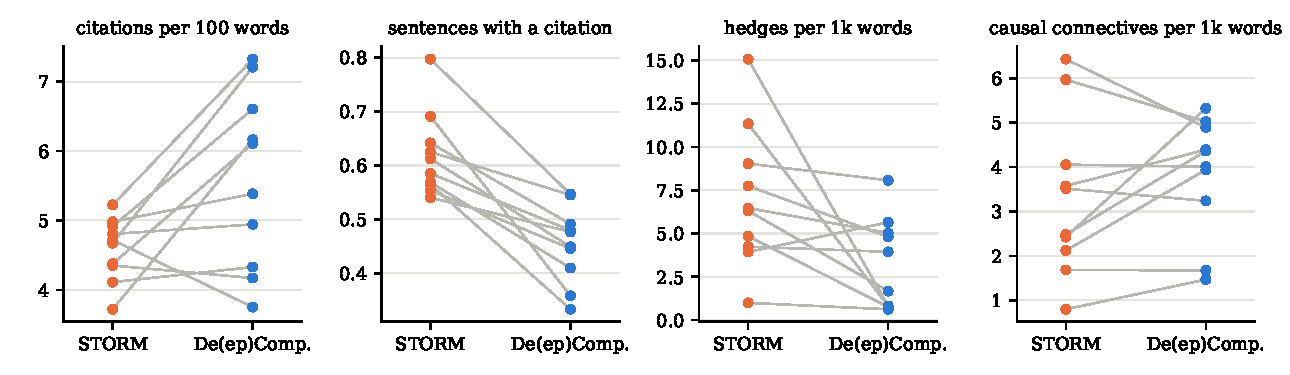
\includegraphics[width=\linewidth]{figs/paired_measures.pdf}
\caption{4 measures per motion, linked across STORM and \sys{}, left to right.}
\label{fig:paired}
\end{figure}

Assuming there is a detectable stance, we would expect it to manifest in the language. Hedges like \emph{may}, \emph{could}, and \emph{suggests} withhold commitment \citep{hyland2005metadiscourse}, whereas markers like \emph{must}, \emph{demonstrates}, and \emph{therefore} assert it. The \sys{} reports use fewer hedges (\txHedgeDc{} per 1{,}000 words versus STORM's \txHedgeSt{} per 1{,}000 words; \sys{} uses fewer on nine of the ten motions; $p = \txHedgeP$) and more commitment markers (\txCommitDc{} versus \txCommitSt{} per 1{,}000 words; \sys{} uses more on all ten motions; $p = \txCommitP$).

Although contrast markers like \emph{however} and \emph{on the other hand} are roughly equivalent (\txContrastDc{} versus \txContrastSt{} per 1{,}000 words; $p = \txContrastP$), so that \sys{} is just as likely to acknowledge the other side, the strength of commitment differs.

Commitment is strongest at the start and weakest at the end of a report. \Cref{tab:stance} provides the side chosen by each \sys{} report, whether the report title makes a claim, and the nature of the conclusion in each report's final paragraph. Nine of ten titles make a claim, as instructed by the prompt. Each of the STORM reports begins with a lead section presenting the question as a debate. The final paragraphs are notably less committed: five firm, two qualifying the claim in the title, two conditionally qualifying it, and one a compromise instead of a yes/no response.

The creativity report concludes that the irreducibility of human creativity persists, ``but only provisionally.'' The theism report concludes that ``the preference for theistic morality depends fundamentally on one's valuation of transcendent moral truth versus pragmatic ethical function.'' One report actually argues against the motion, that application-layer startups will outperform foundation model developers. A plausible explanation is that, although the stance instruction does guide the title and executive summary (both written first), the conclusion is written last from a graph whose branches explore both sides of the question.

The rater marked \sys{} higher on logical connection and attributed this to causal connections between sub-claims. We can use causal connectives like \emph{because}, \emph{leads to}, and \emph{as a result} as a rough proxy. The rate is not reliably different (\sys{}, \txCausalDc{} per 1{,}000 words; STORM, \txCausalSt{} per 1{,}000 words; \sys{} uses more on five motions; $p = \txCausalP$). Note that this captures only a part of logical connection and coherence; we neither refute the rater nor provide independent evidence supporting their claims about a causal chain.

\sys{} reports are more compact than those of STORM: its median report length is \txWordsDc{} words rather than \txWordsSt. It cites more frequently: at \txCiteDensityDc{} citations per 100 words, higher than STORM's \txCiteDensitySt{} ($p = \txCiteDensityP$). However, \sys{} draws on a more restricted range of sources: each \sys{} report cites a median of just \txSourcesDc{} sources, compared with \txSourcesSt{} for STORM. On average, \sys{} cites each source \txCitesPerSourceDc{} times per report, whereas STORM cites each source \txCitesPerSourceSt{} times. In \sys{}, only \txCitedShareDc{} of sentences in each report have citations (compared with \txCitedShareSt{} in STORM).

Rather, the evidence citations are concentrated in bullet points, while the narrative linking those points consists of uncited text. We can see from the bibliographies of \sys{} reports that a large number of retrieved sources will not be cited in the report. The median \sys{} bibliography contains \bibMedDc{} sources (range \bibMinDc--\bibMaxDc), of which just \atUsedMin--\atUsedMax{} are cited (a median of \atUsedShare\%).

\begin{table}[t]
\centering
\small
\begin{tabular}{lrr}
\toprule
Source type & Sources & Share \\
\midrule
Government & 45 & 13\% \\
Academic & 74 & 21\% \\
Think tank or NGO & 78 & 22\% \\
News or magazine & 3 & 1\% \\
Encyclopedia & 4 & 1\% \\
Company, blog, or other & 145 & 42\% \\
\bottomrule
\end{tabular}

\caption{The domains of the \srcN{} sources in ten \sys{} bibliographies, classified by host name.}
\label{tab:sources}
\end{table}

\Cref{tab:sources} provides a domain breakdown of the \srcN{} sources, showing that \srcShareGovernment\% are from government sites, \srcShareAcademic\% from academic (university) sites, \srcShareThinkTankOr\% from think tanks and non-profits and \srcShareCompanyBlogOrOther\% from company sites, blogs and other. There are almost no news sites. We did a test for link validity in October 2026, 11 months after the reports were written: \linkOkPct\% of links resolved correctly, \linkBlockedPct\% refused automation, \linkDeadPct\% had become extinct or returned error. We did not check on STORM's export reports, as they do not include URLs.

In terms of report structure, STORM reports follow the structure of an encyclopedia article: with a short lead section; a background section; sections on arguments for and/or against the motion, often ending with the opposing case. \sys{} reports are written in the form of a brief, with the claim as report title, a short executive summary containing the answer, sections based on branches of the graph, ending with a conclusion. For example, on African Continental Free Trade Area, STORM leads with a description of the agreement and its ratification history, whereas \sys{} leads with the conclusion that ``evidence overwhelmingly supports that its benefits outweigh the harms.''

For the motion that individuals have a moral duty to treat strangers equally to people they know, STORM ends with a description of critics deeming an equal obligation to strangers unrealistic, whereas \sys{} ends with a synthesis of ``impartiality and partiality are not opposites'', which is more moderate than the report title suggests.

\begin{table}[t]
\centering
\small
\begin{tabular}{p{5.2cm}lll}
\toprule
Motion & Side & Title & Final paragraph \\
\midrule
Human creativity will not remain fundamentally irreducible to\,\ldots & for & claim & qualified \\
Individuals have a moral duty to prioritize the well-being of\,\ldots & for & claim & qualified \\
Investing in companies developing foundation models -e.g., OpenAI,\,\ldots & against & claim & firm \\
Israel and Palestine should pursue a long-term joint economic zone\,\ldots & for & claim & firm \\
It is ethically justified for hedge funds to use alternative data\,\ldots & for & topic & conditional \\
Moral systems rooted in theism are preferable to non-theistic\,\ldots & for & claim & conditional \\
The benefits of the African Continental Free Trade Area outweigh\,\ldots & for & claim & firm \\
The U.S. Federal Reserve should prioritize maintaining high\,\ldots & neither & claim & compromise \\
The U.S. should develop wind, solar, and geothermal energy\,\ldots & for & claim & firm \\
U.S. semiconductor manufacturers will outperform global peers over\,\ldots & for & claim & firm \\
\bottomrule
\end{tabular}

\caption{Position of the reported \sys{} reports. We specify the position as it is relative to the wording of the motion: \emph{firm} reports repeat the claims in the motion's title; \emph{qualified} reports restrict these claims; \emph{conditional} reports make them dependent on specific conditions or values that are not part of the motion, and \emph{compromise} reports take a position on neither side.}
\label{tab:stance}
\end{table}
